% Document packages / layout
\documentclass[
    pdf,
    11pt,
    xcolor={svgnames},
    %hyperref={colorlinks, citecolor=Cyan, linkcolor=Cyan, urlcolor=Cyan}
  ]{beamer}
%\usetheme{Copenhagen}
\usetheme{Madrid}
\usecolortheme{beaver}
\usepackage{color}

\usepackage[style=alphabetic]{biblatex}
\addbibresource{citations.bib}

% Remove navigation controls
\setbeamertemplate{navigation symbols}{}

% Un-numbered footnote
\newcommand\blfootnote[1]{%
  \begingroup
  \renewcommand\thefootnote{}\footnote{\scriptsize #1}%
  \addtocounter{footnote}{-1}%
  \endgroup
}

% Figure Packages
\usepackage{float}
\usepackage{subcaption}

% Math Packages
\usepackage{amsmath,amsthm,amssymb,mathrsfs,bm}
\usepackage{commath}
\usepackage{physics}

% Quality of Life Packages
\usepackage{enumerate}
\usepackage{siunitx} %\sisetup{inter-unit-product =$\cdot$}
\usepackage{multicol}
\usepackage{wrapfig}
\usepackage{graphicx}

%\newtheorem*{definition}{Definition}

% Creates section subdivider at beginning of each section.
\AtBeginSection[]
{
  \begin{frame}
    \frametitle{Table of Contents}
    \tableofcontents[currentsection]
  \end{frame}
}
 
\title[WBSG for Random Scalar Hyperbolic Laws]{%
  A Well-Balanced Stochastic Galerkin Method for Scalar Hyperbolic Laws with Random Forcing.
}
\author[Chowdhary, Shedlock]{%
  Andrew Shedlock and Abhijit Chowdhary
}
\institute[NCSU]{
  Department of Mathematics \\
  North Carolina State University
}
\date[MA788 NCSU]{\today}

\begin{document}

\frame{ \titlepage }

\begin{frame}
\begin{figure}
\centering
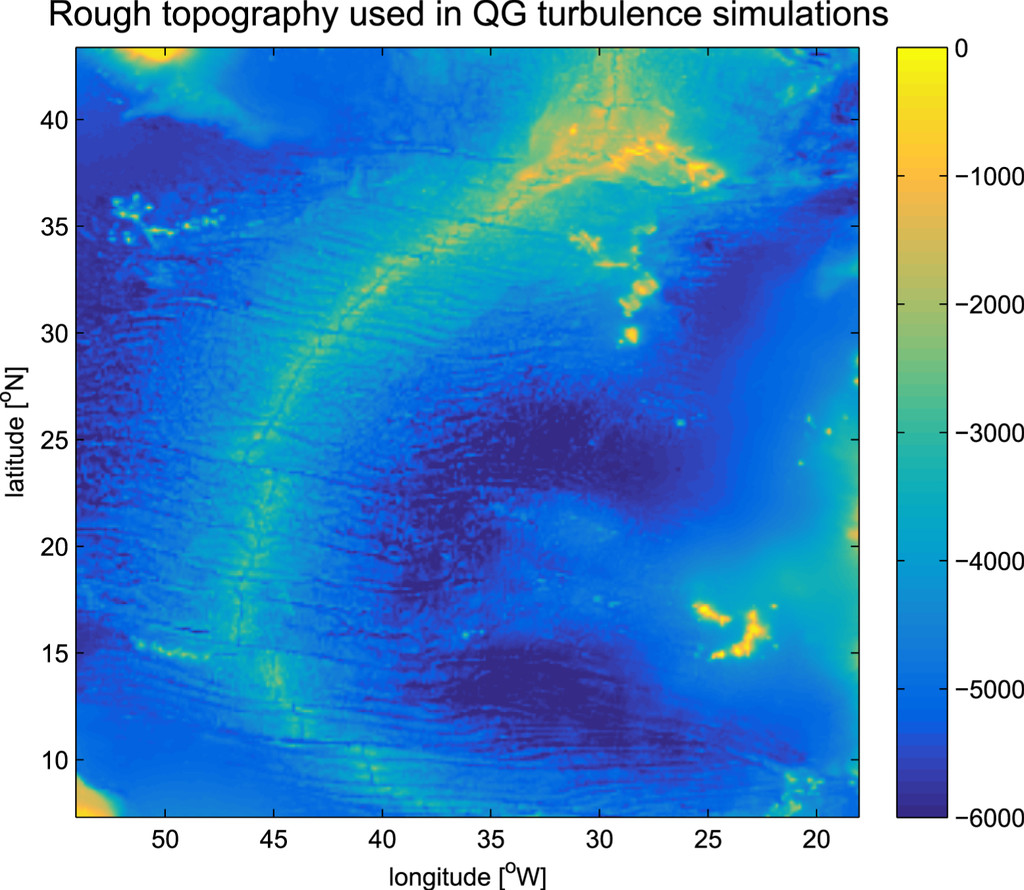
\includegraphics[width=0.70\textwidth]{slides/bottom_topography.jpg}
\end{figure}
\blfootnote{\fullcite{Trossman2017}}
\end{frame}

\begin{frame}
    \frametitle{Difficulties in real-world simulation}
    \begin{columns}
    \begin{column}{0.5\textwidth}
    If the given bottom topography given was our source term, we would have:
    \vspace{-1em}
    \begin{itemize}
        \item Uncertainty in measurement
        \item Low regularity
    \end{itemize}
    The former can have a non-negligible effect on simulation and the latter can pose difficulties in capturing the true steady state solution.
    \end{column}
    \begin{column}{0.5\textwidth}
        \begin{figure}
        \centering
        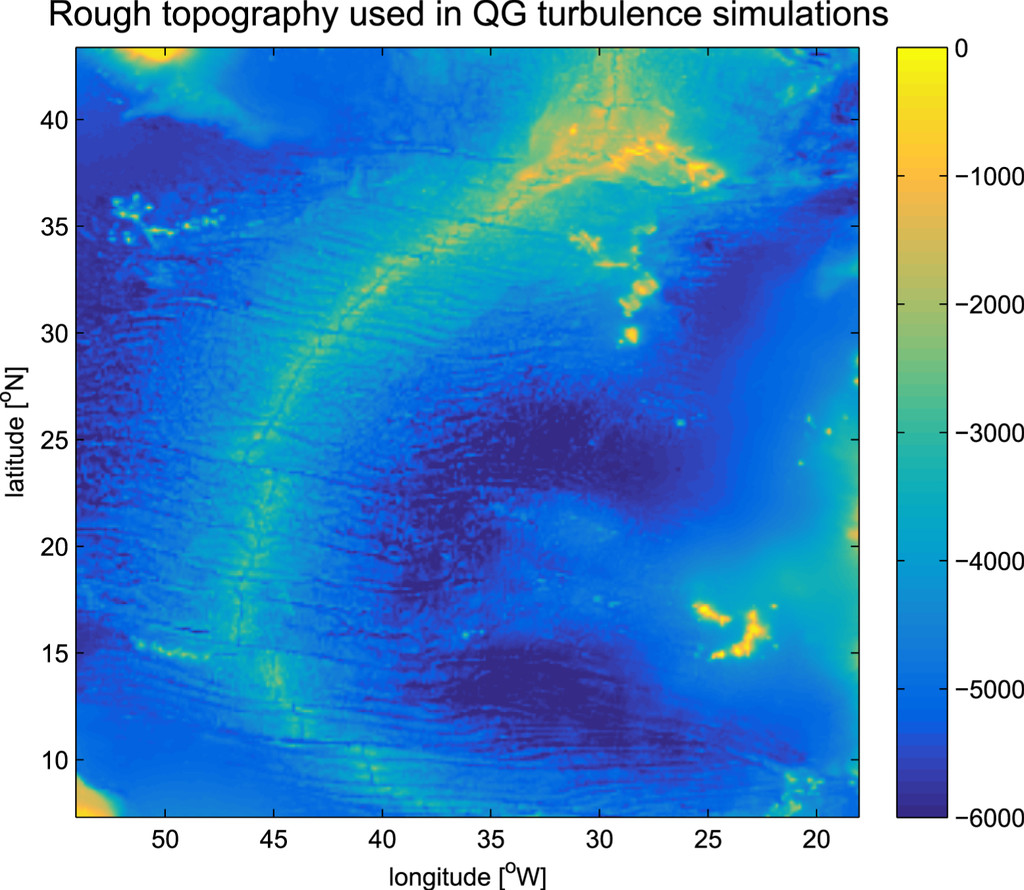
\includegraphics[width=\textwidth]{slides/bottom_topography.jpg}
        \end{figure}
    \end{column}
    \end{columns}
    {\bf Idea:} Combine previous ideas for stochastic Galerkin via generalized polynomial chaos and well-balanced interface methods.
    \blfootnote{\fullcite{Jin2015}}
\end{frame}

%%%%%%%%%%%%%%%%%%%%%%%%%%%%%%%%%%%%%%%%%%%%%%%%%%%%%%%%%%%%%%%%%%%%%%%%%%%%%%%
%%% Preliminaries
%%%%%%%%%%%%%%%%%%%%%%%%%%%%%%%%%%%%%%%%%%%%%%%%%%%%%%%%%%%%%%%%%%%%%%%%%%%%%%%
\section{Stochastic Galerkin and an Initial Attempt}

\begin{frame}{Introduction to stochastic Galerkin via gPC}
    Consider a general SDE with random inputs:
    \begin{equation} \label{eq:SDE}
        \partial_t u = \mathcal{L}(t,x,u,z;b(x,z))
    \end{equation}
    where, for convenience, let $z \in I_z \subset \mathbb{R}$ parameterize the random input.
    
    \pause
    
    We seek to approximate $u$ with the gPC expansion:
    \begin{align*}
        u(x,t,z) &= u_M(x,t,z) = \sum_{m=1}^M \hat{u}_m(t,x) \Phi_m(z) \\
        b(x,z) &= u_M(x,z) = \sum_{m=1}^M \hat{b}_m(t,x) \Phi_m(z) 
    \end{align*}
    where $\{\Phi_m(z)\} \subset \mathbb{P}_M$ are the orthonormal polynomials satisfying
    \[
    \int \Phi_i(z) \Phi_j(z) \rho(z) \dd{z} = \delta_{ij},
    \quad 1 \leq i,j \leq M
    \]
\end{frame}

\begin{frame}{Naive Stochastic Galerkin for Burgers}
    Let's focus on Burgers' equation with a random source term
    \begin{equation}
        \partial_t u + \partial_x \left( \frac{u^2}{2} \right) = -b'(x,z) u
    \end{equation}
    \pause
    Consider the uniform discretization:
    \begin{itemize}
        \item $(x_{j+1/2})_{j=1}^{N_x}$ with $\Delta x = x_{j+1/2}-x_{j-1/2}$;
        \item $(t_n)_{n=1}^{N_t}$ with $\Delta t = t^n - t^{n-1}$.
    \end{itemize}
    with:
    \begin{equation*}
        u_j^n = \frac{1}{\Delta x} \int_{x_{j-1/2}}^{x_{j+1/2}} u(x,t^n) \dd{x}
    \end{equation*}
    \pause
    A natural way to discretize Burgers is:
    \begin{equation} \label{eq:burgers_inteface}
        \partial_t u_j + \frac{u_j^2 - u_{j-1}^2}{2 \Delta x} = -\frac{b_j - b_{j-1}}{\Delta x} u_j
    \end{equation}
    where we've applied an upwind flux assuming $u > 0$ for brevity.
\end{frame}

\begin{frame}{Naive Stochastic Galerkin for Burgers}
    Multiplying both sides of the discretization by $\Phi_j$ and taking an expectation:
    \begin{multline*}
        \mathbb{E}\left[
            \left(
                \pdv{}{t} u_{M,j} + \frac{u_{M,j}^2-u_{N,j-1}^2}{2\Delta x}
            \right) \Phi_m(z)
        \right] \\
        = -\mathbb{E} \left[
            \frac{b_{M,j} - b_{M,j-1}}{\Delta x} u_{M,j} \Phi_m(z)
        \right]
    \end{multline*}
    \pause
    Finally, substitute in their gPC expansions and and use orthonormality:
\end{frame}
\begin{frame}{Naive Stochastic Galerkin for Burgers}
   \begin{equation}
       \partial_t \hat{\vb{u}}_j + \frac{\vb{A}_j \hat{\vb{u}}_j - \vb{A}_{j-1} \hat{\vb{u}}_{j-1}}{2\Delta x} = -\frac{(\vb{B}_j - \vb{B}_{j-1})}{2\Delta x}\hat{\vb{u}}_j
   \end{equation} 
   where:
   \begin{equation*}
       \hat{\vb{u}} = (\hat{u}_1, \dots, \hat{u}_M)^\mathrm{T}
       \qquad
       \hat{\vb{b}} = (\hat{b}_1, \dots, \hat{b}_M)^\mathrm{T}
   \end{equation*}
   \begin{align*}
       [\vb{A}_j]_{mn} &= \mathbb{E}[u_{N,j} \Phi_m \Phi_n] = \sum_{k=1}^M \hat{u}_{k,j} e_{kmn} \\
       [\vb{B}_j]_{mn} &= \mathbb{E}[b_{N,j} \Phi_m \Phi_n] = \sum_{k=1}^M \hat{b}_{k,j} e_{kmn}
   \end{align*}
   with $e_{kmn} = \mathbb{E}[\Phi_k \Phi_m \Phi_n]$.
\end{frame}

\begin{frame}{Test Problems}
    Impose the following initial/boundary conditions:
    \[
    \begin{cases}
        u(x,0) = 0, &\forall x > 0 \\
        u(0,t) = 2, &\forall t > 0
    \end{cases}
    \]
    With the following bottom functions:
    \begin{align*}
        b_1(x,z)
        &=
        \begin{cases}
            (2+z) \cos(\pi x), & 4.5 \leq x \leq 5.5 \\
            0, & \text{otherwise}
        \end{cases} \\
        b_2(x,z)
        &=
        \begin{cases}
            0.1(2+z) \cos(\pi x), & 5 \leq x \leq 6 \\
            0, & \text{otherwise}
        \end{cases}
    \end{align*}
    {\bf Note:}, $b_1$ is continuous and $b_2$ is discontinuous.
\end{frame}

\begin{frame}{Mean: Why well-balanced matters}
    \begin{figure}
    \centering
    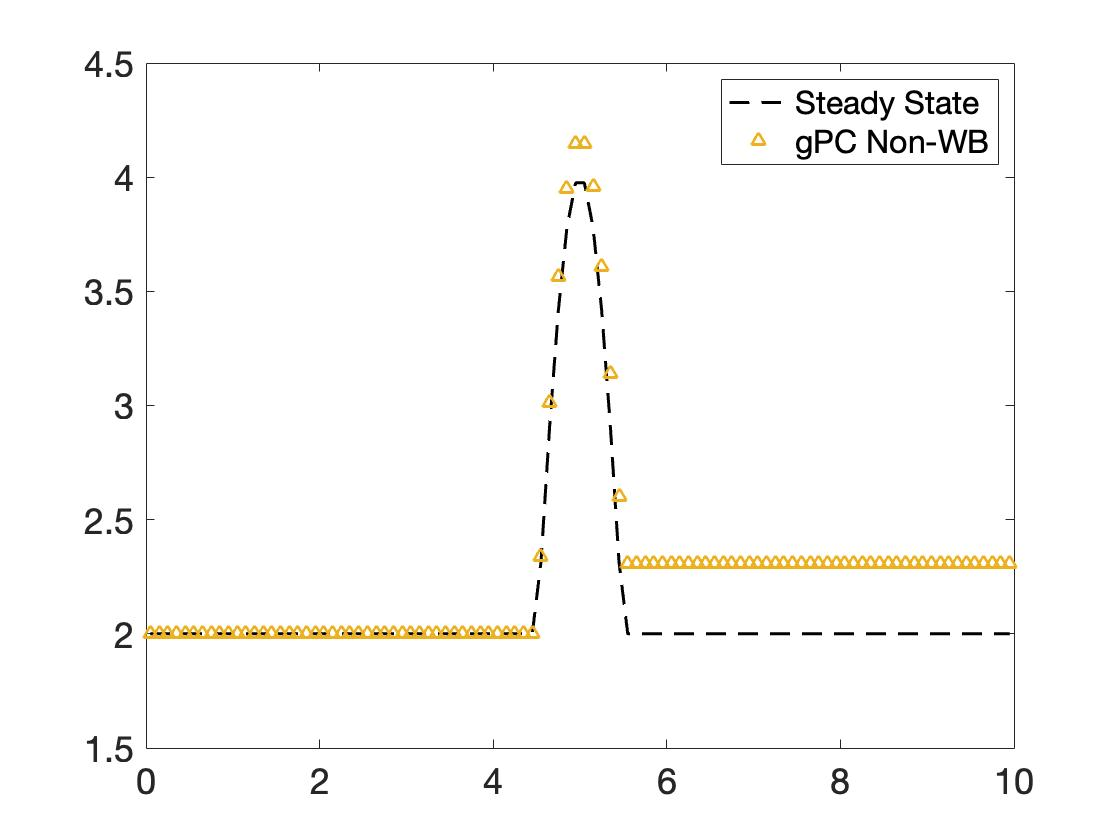
\includegraphics[width=0.85\textwidth]{./Figures/burgers_non_mean}
    \end{figure}
\end{frame}
\begin{frame}{Standard Deviation: Why well-balanced matters}
    \begin{figure}
    \centering
    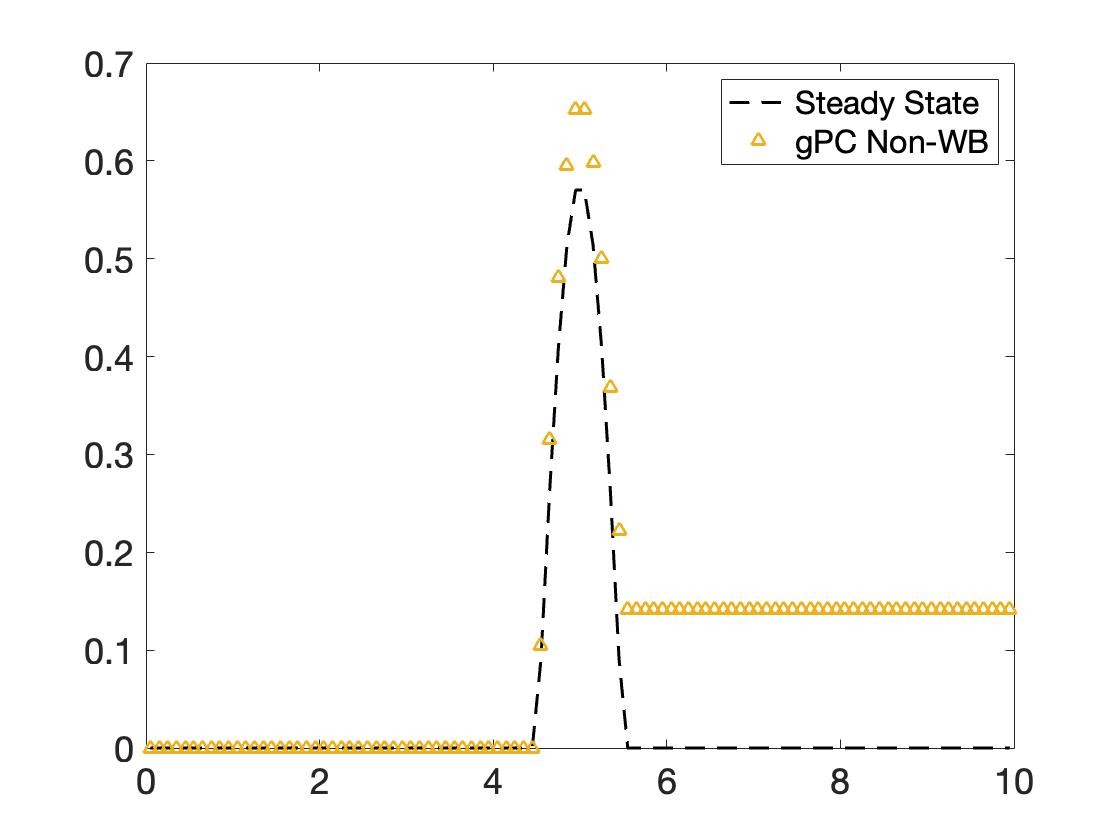
\includegraphics[width=0.85\textwidth]{./Figures/burgers_non_sd}
    \end{figure}
\end{frame}
\begin{frame}{Mean: Discontinuous bottom topography}
    \begin{figure}
    \centering
    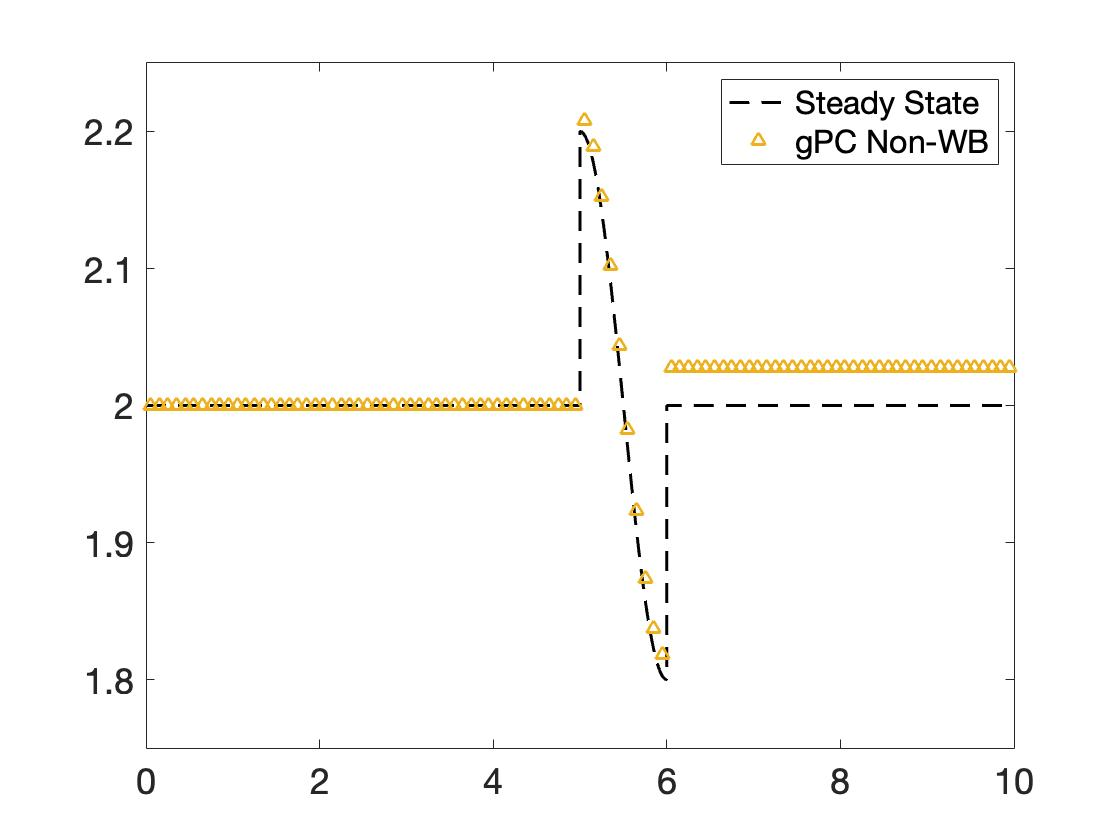
\includegraphics[width=0.85\textwidth]{./Figures/burgers_dis_non_mean}
    \end{figure}
\end{frame}
\begin{frame}{Standard Deviation: Discontinuous bottom topography}
    \begin{figure}
    \centering
    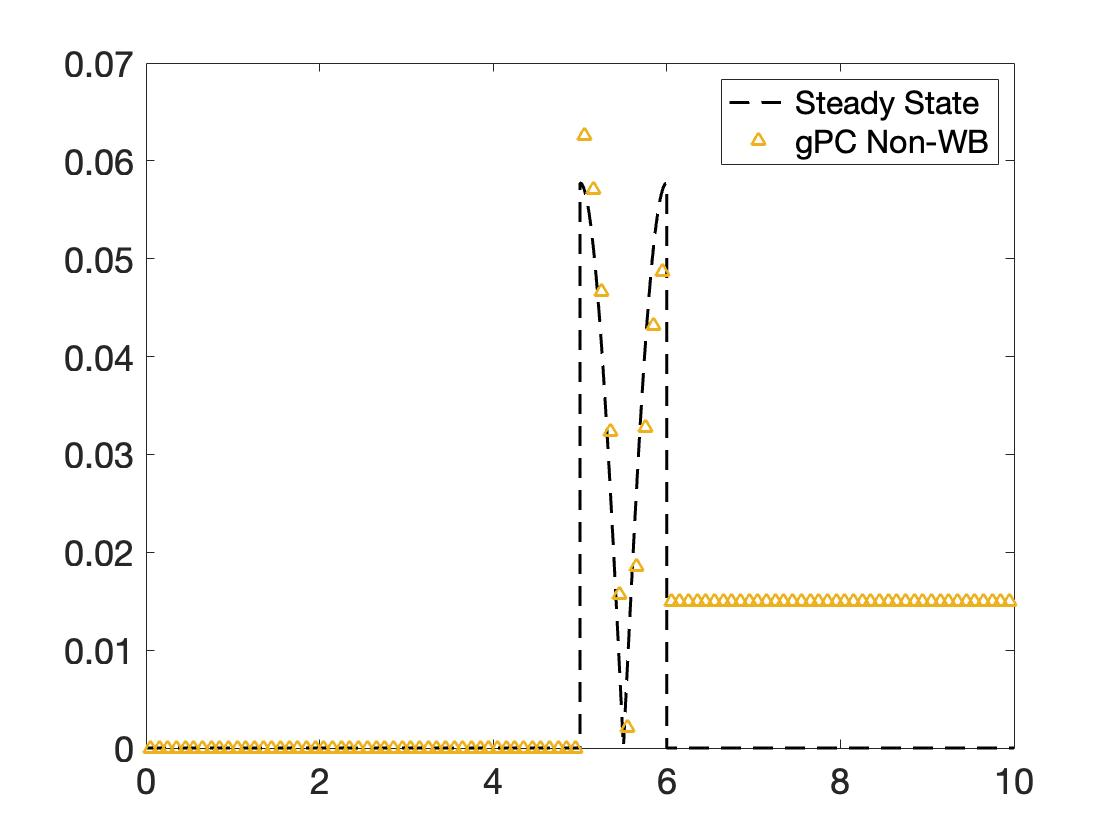
\includegraphics[width=0.85\textwidth]{./Figures/burgers_dis_non_sd}
    \end{figure}
\end{frame}

%%%%%%%%%%%%%%%%%%%%%%%%%%%%%%%%%%%%%%%%%%%%%%%%%%%%%%%%%%%%%%%%%%%%%%%%%%%%%%%
%%% Remarks on Well-Balanced Schemes
%%%%%%%%%%%%%%%%%%%%%%%%%%%%%%%%%%%%%%%%%%%%%%%%%%%%%%%%%%%%%%%%%%%%%%%%%%%%%%%
\section{Remarks on Well-Balanced Schemes}

\begin{frame}{Determininistic Model Problem}
    Given the scalar conservation law with source term:
    \begin{equation} \label{eq:model}
        \partial_t u + \partial_x f(u) = -b'(x) q(u).
    \end{equation}
    we have the steady-state equation
    \begin{equation} \label{eq:model_ss}
         \partial_x f(u) + -b'(x) q(u) = 0.
    \end{equation}
    which, supposing a smooth solution, can be written into the form:
    \begin{equation} \label{eq:ss_condition}
        \begin{cases}
            D(x) + b(x) = {\rm constant}. \\
            D(x) = \int_0^{u(x)} \frac{f'(s)}{q(s)} \dd{s}
        \end{cases}
    \end{equation}
    which we call the steady-state condition.
\end{frame}

\subsection{A Well-Balanced Deterministic Scheme}
\begin{frame}{A Well-Balanced Numerical Scheme}
    \begin{definition}
        A numerical scheme is called well-balanced (WB) if it can preserve the steady-state condition \eqref{eq:ss_condition} either exactly, or formally with at least second order accuracy.
    \end{definition}
    \pause
    Construct the semi-discrete interface method proposed in \cite{Jin2001}:
    \begin{equation}
        \partial_t u_j + \frac{f_{j+1/2} - f_{j-1/2}}{\Delta x} = - \frac{b_{j+1/2} - b_{j-1/2}}{\Delta x} 
        \underbrace{\frac{q_{j+1/2} + q_{j-1/2}}{2}}_{\text{Critical Difference}}
    \end{equation}
    \pause
    or if $D(x)$ is monotone: (Recall:$D = \int_0^{u(x)} f'(s)/q(s) \dd{s}$)
    \begin{equation} \label{eq:deterministic_scheme}
        \partial_t u_j + \frac{f_{j+1/2} - f_{j-1/2}}{\Delta x} = - \frac{b_{j+1/2} - b_{j-1/2}}{\Delta x} \frac{f_{j+1/2} + f_{j-1/2}}{D_{j+1/2}-D_{j-1/2}}
    \end{equation}
\end{frame}

% Pause is broken in align 
% https://tex.stackexchange.com/questions/6348/problem-with-beamers-pause-in-alignments
\begin{frame}
    Hence, considering the steady state solution:
    \begin{align*}
        & 
        \frac{f_{j+1/2} - f_{j-1/2}}{\Delta x} + \frac{b_{j+1/2} - b_{j-1/2}}{\Delta x} \frac{f_{j+1/2} + f_{j-1/2}}{D_{j+1/2}-D_{j-1/2}} = 0
    \end{align*}
\end{frame}
\begin{frame}
    Hence, considering the steady state solution:
    \begin{align*}
        & 
        \frac{f_{j+1/2} - f_{j-1/2}}{\Delta x} + \frac{b_{j+1/2} - b_{j-1/2}}{\Delta x} \frac{f_{j+1/2} + f_{j-1/2}}{D_{j+1/2}-D_{j-1/2}} = 0 \\
        \implies\ 
        &
        D_{j+1/2} - D_{j-1/2} + b_{j+1/2} - b_{j-1/2} = 0
    \end{align*}
\end{frame}
\begin{frame}
    Hence, considering the steady state solution:
    \begin{align*}
        & 
        \frac{f_{j+1/2} - f_{j-1/2}}{\Delta x} + \frac{b_{j+1/2} - b_{j-1/2}}{\Delta x} \frac{f_{j+1/2} + f_{j-1/2}}{D_{j+1/2}-D_{j-1/2}} = 0 \\
        \implies\ 
        &
        D_{j+1/2} - D_{j-1/2} + b_{j+1/2} - b_{j-1/2} = 0 \\
        \implies\ 
        &
        D_{j+1/2} + b_{j+1/2} = {\rm constant}
    \end{align*}
    The steady state condition \eqref{eq:ss_condition} is preserved {\em exactly} at the cell interface!
\end{frame}

\subsection{Extension to Stochastic Galerkin Setting}

\begin{frame}{Stochastic Well-Balanced Schemes}
    \begin{block}{Stochastic WB}
        Let $\mathcal{S}$ be a numerical scheme for \eqref{eq:sburgers}, which results in a solution $v(z) \in V_z$, where $V_z$ is a finite dimensional linear function space.
        \begin{itemize}
            \item  A numerical scheme $\mathcal{S}$ is called {\em strongly well-balanced} if it preserves the steady state condition either exactly or formally with at least second order accuracy for almost every $z$.
            \item It is {\em weakly well-balanced} if it satisfies the weak form of the steady state (in the sense of Galerkin) with at least second order accuracy.
        \end{itemize}
    \end{block}
    \pause
    \textbf{Claim:} The previous interface method will be well-balanced for Burgers.
\end{frame}

%%%%%%%%%%%%%%%%%%%%%%%%%%%%%%%%%%%%%%%%%%%%%%%%%%%%%%%%%%%%%%%%%%%%%%%%%%%%%%%
%%% Stochastic WB scheme for Burgers
%%%%%%%%%%%%%%%%%%%%%%%%%%%%%%%%%%%%%%%%%%%%%%%%%%%%%%%%%%%%%%%%%%%%%%%%%%%%%%%
\section{A sWB scheme for Burgers' equation}

\begin{frame}{Burgers' equation}
    Consider Burgers' equation with a random source term
    \begin{equation} \label{eq:sburgers}
        \partial_t u + \partial_x \left( \frac{u^2}{2} \right) = -b'(x,z) u
    \end{equation}
    \pause
    We apply the interface method to find
    \begin{equation} \label{eq:burgers_inteface}
        \partial_t u_j + \frac{u_j^2 - u_{j-1}^2}{2 \Delta x} = -\frac{b_j - b_{j-1}}{\Delta x} \frac{u_j + u_{j-1}}{2}
    \end{equation}
    where we've applied an upwind flux assuming $u > 0$ for brevity.
\end{frame}

\begin{frame}{sWB Burgers}
    Multiplying both sides of the discretization by $\Phi_j$ and taking an expectation:
    \begin{multline*}
        \mathbb{E}\left[
            \left(
                \pdv{}{t} u_{N,j} + \frac{u_{N,j}^2-u_{N,j-1}^2}{2\Delta x}
            \right) \Phi_m(z)
        \right] \\
        = -\mathbb{E} \left[
            \Big(\frac{b_{N,j} - b_{N,j-1}}{\Delta x}\Big)\Big( \frac{u_{N,j} - u_{N,j-1}}{2}\Big) \Phi_m(z)
        \right]
    \end{multline*}
    Finally, substitute in their gPC expansions and and use orthonormality:
\end{frame}

\begin{frame}{sWB Burgers Full Scheme}
   \begin{equation}
       \partial_t \hat{\vb{u}}_j + \frac{\vb{A}_j \hat{\vb{u}}_j - \vb{A}_{j-1} \hat{\vb{u}}_{j-1}}{2\Delta x} = -\frac{(\vb{B}_j - \vb{B}_{j-1})(\hat{\vb{u}}_j + \hat{\vb{u}}_{j-1})}{2\Delta x}
   \end{equation} 
   where:
   \begin{equation*}
       \hat{\vb{u}} = (\hat{u}_1, \dots, \hat{u}_M)^\mathrm{T}
       \qquad
       \hat{\vb{b}} = (\hat{b}_1, \dots, \hat{b}_M)^\mathrm{T}
   \end{equation*}
   \begin{align*}
       [\vb{A}_j]_{mn} = [\vb{A}(\hat{\vb{u}}_j)] &= \mathbb{E}[u_{M,j} \Phi_m \Phi_n] = \sum_{k=1}^M \hat{u}_{k,j} e_{kmn} \\
       [\vb{B}_j]_{mn} = [\vb{A}(\hat{\vb{b}}_j)] &= \mathbb{E}[b_{M,j} \Phi_m \Phi_n] = \sum_{k=1}^M \hat{b}_{k,j} e_{kmn}
   \end{align*}
   with $e_{kmn} = \mathbb{E}[\Phi_k \Phi_m \Phi_n]$.
\end{frame}

\begin{frame}
   The steady state governing equation is:
   \[
   \partial_x ( u^2/2 ) + b'(x,z) u = 0
   \]
   which, under it's gPC approximation goes to:
   \[
   \mathbb{E}\left[
        ( u_M^2/2 )_x \Phi_m
   \right]
   = - \mathbb{E}\left[
        ( b_M )_x u_M \Phi_m
   \right]
   \implies
   \pdv{}{x} \/ (\vb{A} \vb{u}) + \vb{B}'(x) \vb{u} = 0
   \]
   \pause
    Our scheme:
   \begin{equation*}
       \partial_t \hat{\vb{u}}_j + \frac{\vb{A}_j \hat{\vb{u}}_j - \vb{A}_{j-1} \hat{\vb{u}}_{j-1}}{2\Delta x} = -\frac{(\vb{B}_j - \vb{B}_{j-1})(\hat{\vb{u}}_j + \hat{\vb{u}}_{j-1})}{2\Delta x}
   \end{equation*} 
   reduces to
   \begin{equation*}
       \frac{\vb{A}_j \hat{\vb{u}}_j - \vb{A}_{j-1} \hat{\vb{u}}_{j-1}}{2\Delta x} + \frac{(\vb{B}_j - \vb{B}_{j-1})(\hat{\vb{u}}_j + \hat{\vb{u}}_{j-1})}{2\Delta x} = 0
   \end{equation*} 
   This is sWB via the same procedure as the deterministic system.
\end{frame}


%%%%%%%%%%%%%%%%%%%%%%%%%%%%%%%%%%%%%%%%%%%%%%%%%%%%%%%%%%%%%%%%%%%%%%%%%%%%%%%
%%% Results
%%%%%%%%%%%%%%%%%%%%%%%%%%%%%%%%%%%%%%%%%%%%%%%%%%%%%%%%%%%%%%%%%%%%%%%%%%%%%%%
\section{Results}

\begin{frame}{Test Problems}
    Impose the following initial/boundary conditions:
    \[
    \begin{cases}
        u(x,0) = 0, &\forall x > 0 \\
        u(0,t) = 2, &\forall t > 0
    \end{cases}
    \]
    With the following bottom functions:
    \begin{align*}
        b_1(x,z)
        &=
        \begin{cases}
            (2+z) \cos(\pi x), & 4.5 \leq x \leq 5.5 \\
            0, & \text{otherwise}
        \end{cases} \\
        b_2(x,z)
        &=
        \begin{cases}
            0.1(2+z) \cos(\pi x), & 5 \leq x \leq 6 \\
            0, & \text{otherwise}
        \end{cases}
    \end{align*}
    {\bf Note:}, $b_1$ is continuous and $b_2$ is discontinuous.
\end{frame}

\begin{frame}{Mean: Why well-balanced matters}
    \begin{figure}
    \centering
    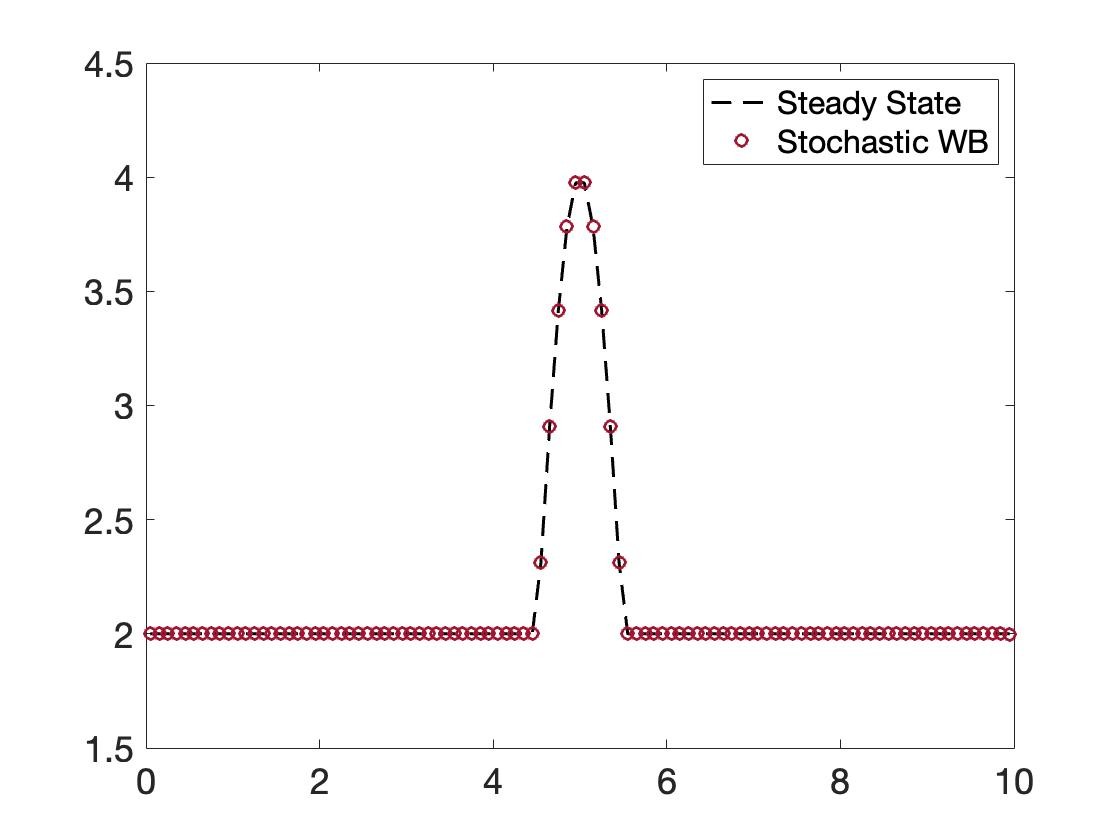
\includegraphics[width=0.85\textwidth]{./Figures/burgers_wb_mean}
    \end{figure}
\end{frame}
\begin{frame}{Mean: Why well-balanced matters}
    \begin{figure}
    \centering
    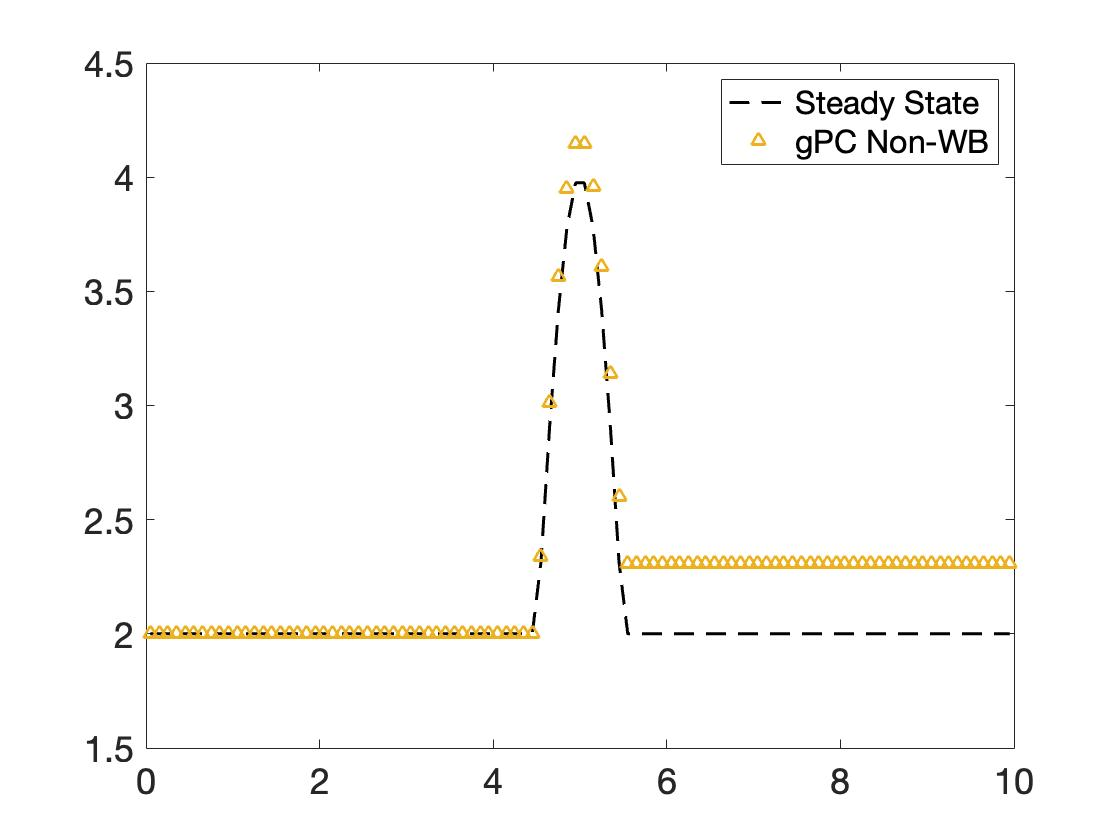
\includegraphics[width=0.85\textwidth]{./Figures/burgers_non_mean}
    \end{figure}
\end{frame}

\begin{frame}{Standard Deviation: Why well-balanced matters}
    \begin{figure}
    \centering
    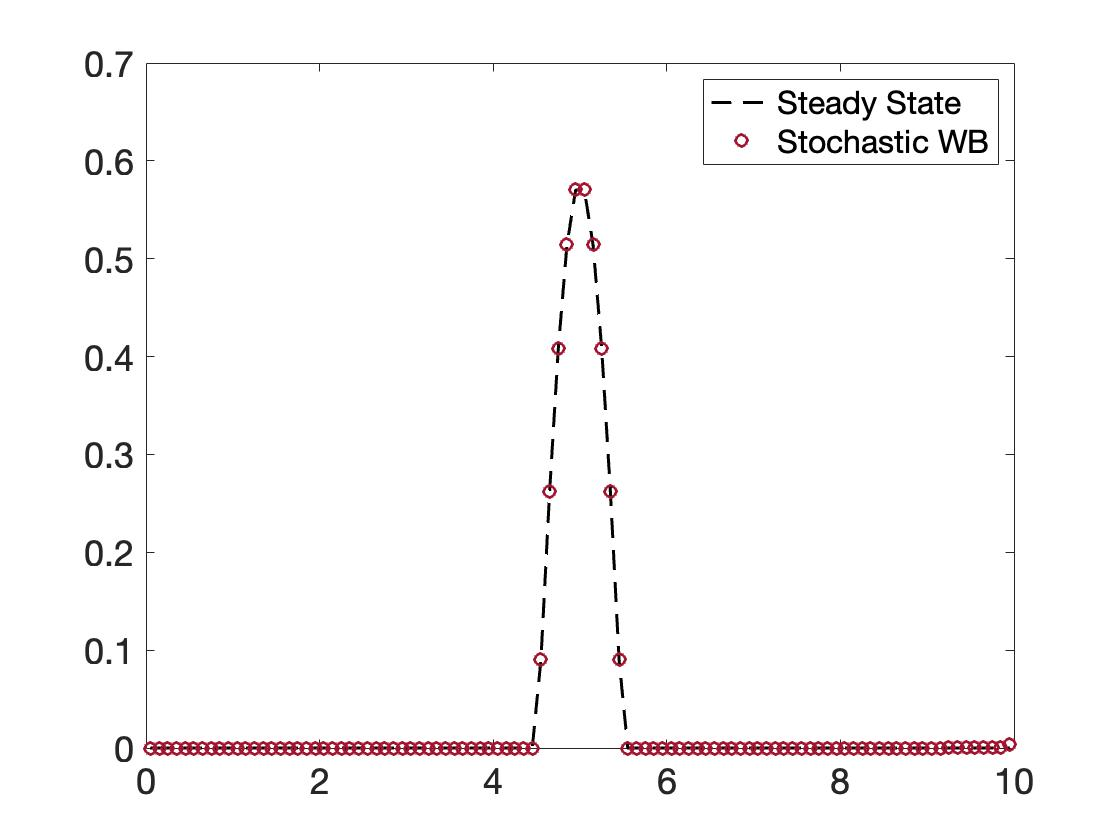
\includegraphics[width=0.85\textwidth]{./Figures/burgers_wb_sd}
    \end{figure}
\end{frame}
\begin{frame}{Standard Deviation: Why well-balanced matters}
    \begin{figure}
    \centering
    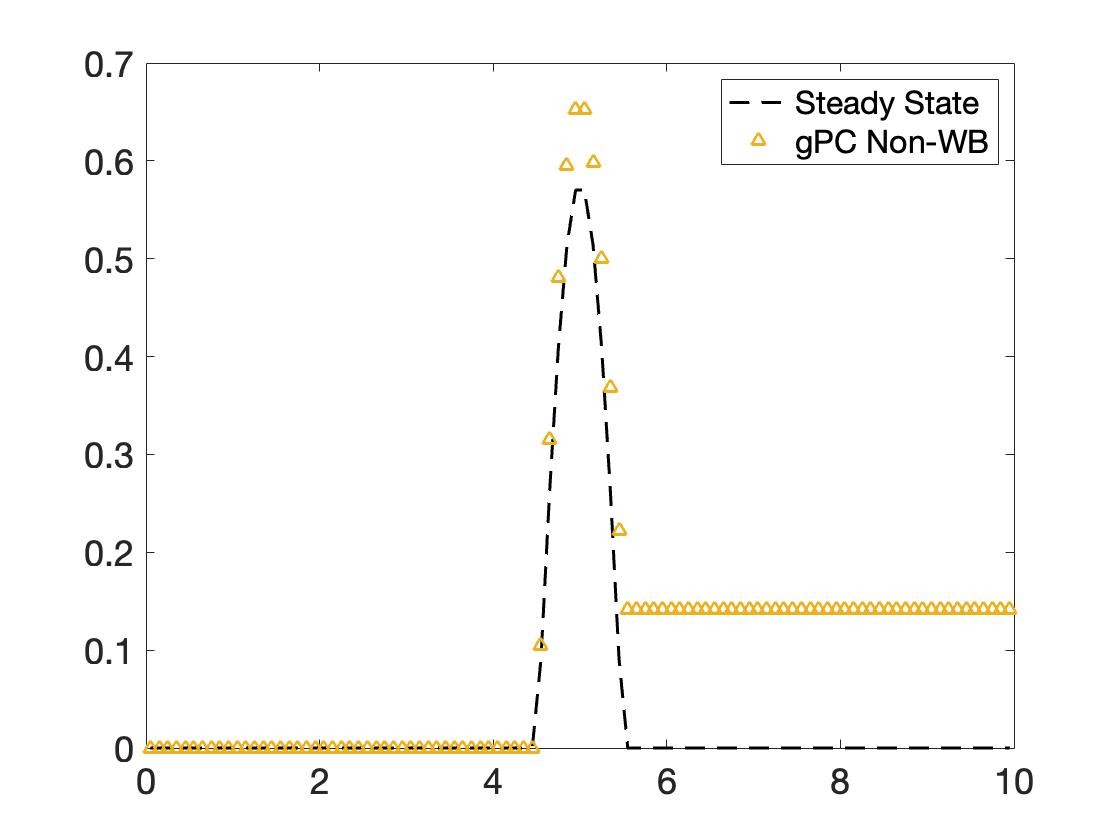
\includegraphics[width=0.85\textwidth]{./Figures/burgers_non_sd}
    \end{figure}
\end{frame}

\begin{frame}{Mean: Discontinuous bottom topography}
    \begin{figure}
    \centering
    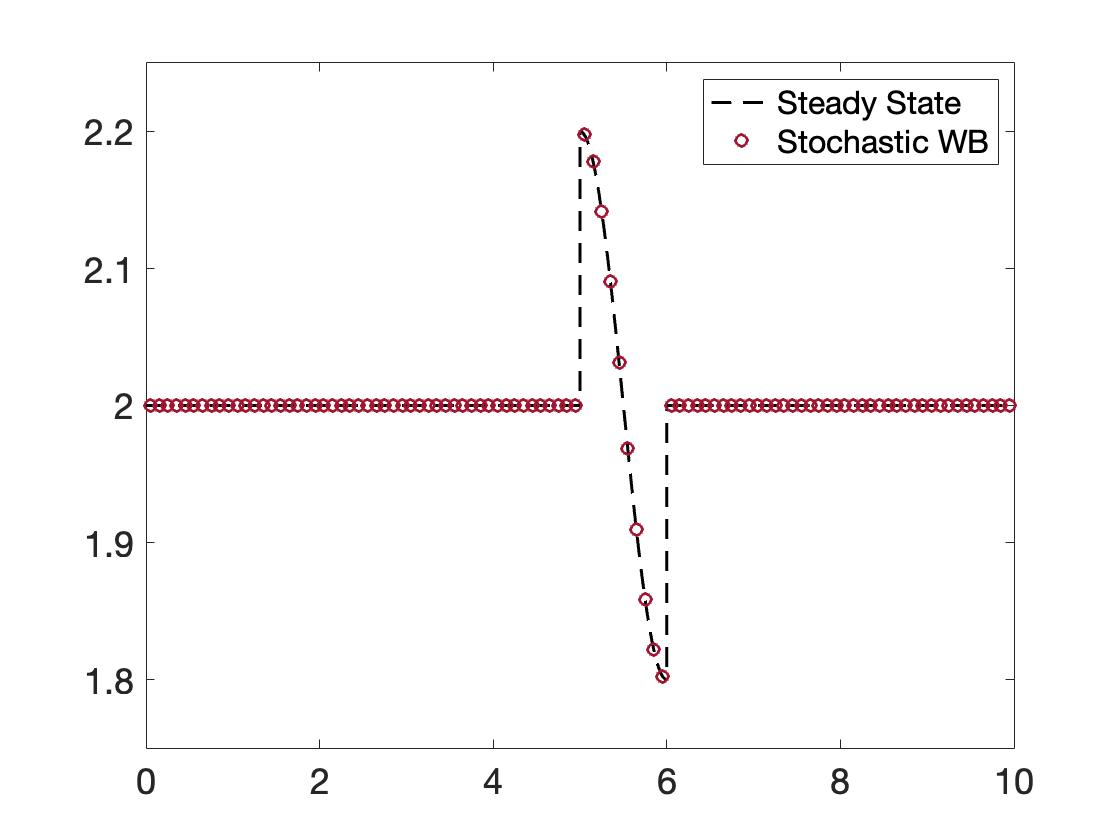
\includegraphics[width=0.85\textwidth]{./Figures/burgers_dis_wb_mean}
    \end{figure}
\end{frame}
\begin{frame}{Mean: Discontinuous bottom topography}
    \begin{figure}
    \centering
    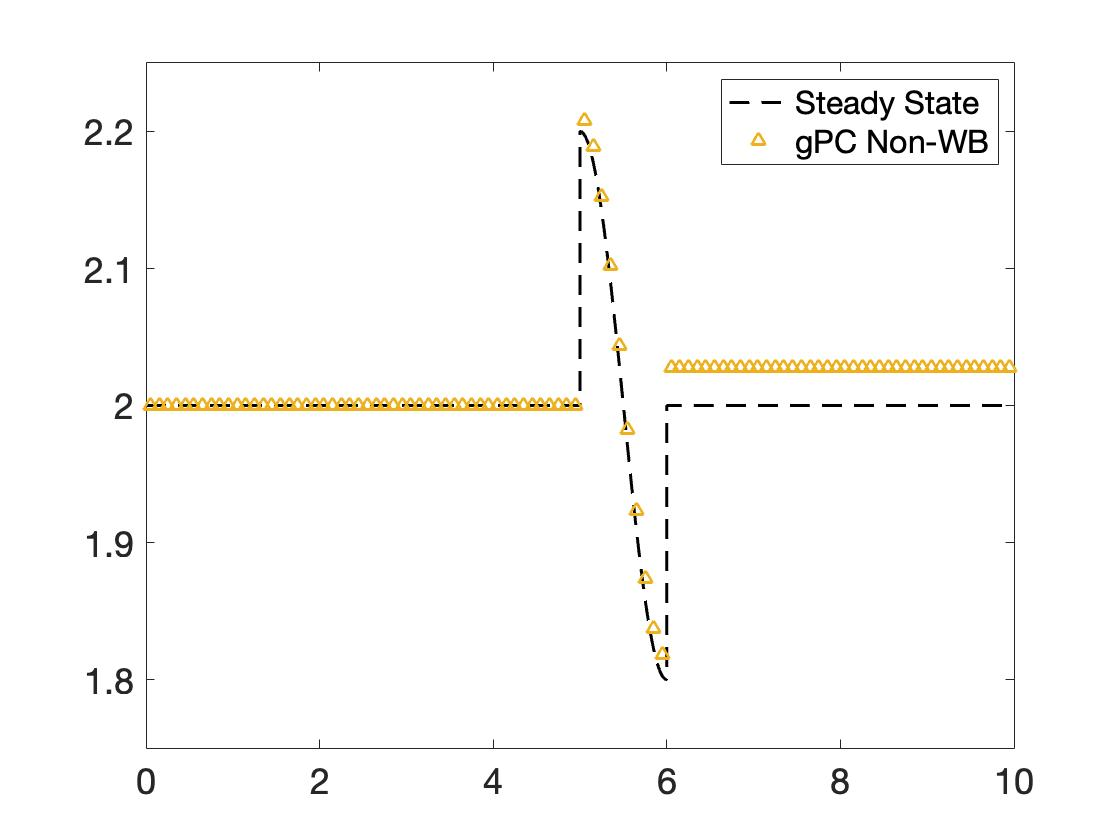
\includegraphics[width=0.85\textwidth]{./Figures/burgers_dis_non_mean}
    \end{figure}
\end{frame}

\begin{frame}{Standard Deviation: Discontinuous bottom topography}
    \begin{figure}
    \centering
    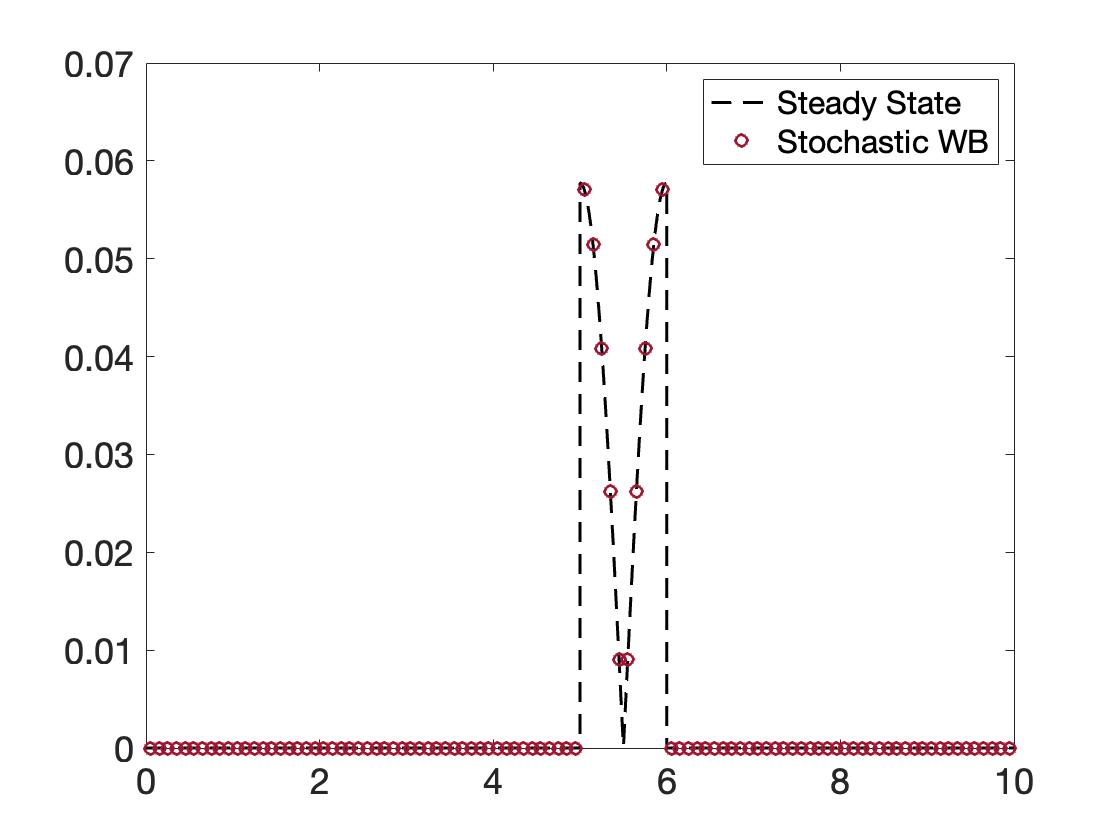
\includegraphics[width=0.85\textwidth]{./Figures/burgers_dis_wb_sd}
    \end{figure}
\end{frame}
\begin{frame}{Standard Deviation: Discontinuous bottom topography}
    \begin{figure}
    \centering
    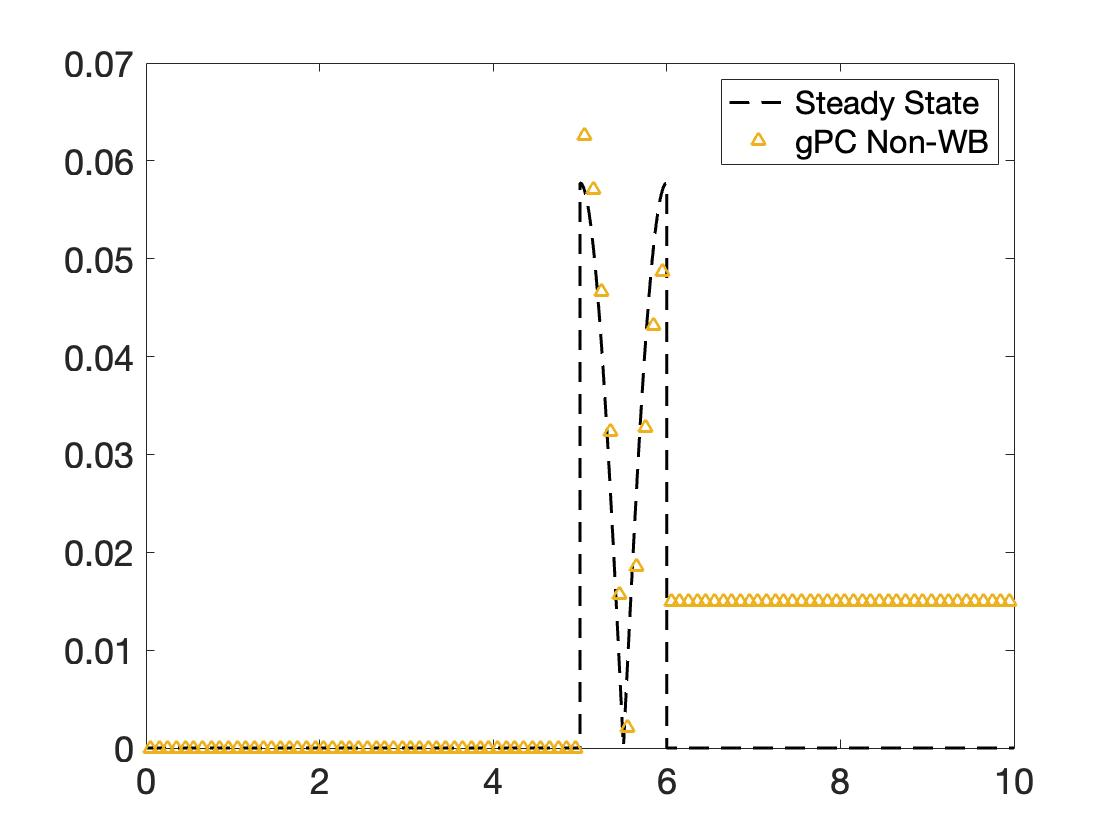
\includegraphics[width=0.85\textwidth]{./Figures/burgers_dis_non_sd}
    \end{figure}
\end{frame}

\begin{frame}{An alternative flux}
    Likewise, with flux $f(u) = u^4 / 4$ we can derive a similar method:
   \begin{equation}
       \partial_t \hat{\vb{u}}_j + \frac{\vb{S}_j \hat{\vb{u}}_j - \vb{S}_{j-1} \hat{\vb{u}}_{j-1}}{4\Delta x} = -\frac{(\vb{B}_j - \vb{B}_{j-1})(\hat{\vb{u}}_j + \hat{\vb{u}}_{j-1})}{2\Delta x}
   \end{equation} 
   where:
   \begin{equation*}
       \hat{\vb{u}} = (\hat{u}_1, \dots, \hat{u}_M)^\mathrm{T}
       \qquad
       \hat{\vb{b}} = (\hat{b}_1, \dots, \hat{b}_M)^\mathrm{T}
   \end{equation*}
   \begin{align*}
       [\vb{S}_j]_{mn} &= \mathbb{E}[u_{N,j}^3 \Phi_m \Phi_n]  = \sum_{p,q,r}^M \hat{u}_{p,j} \hat{u}_{q,j} \hat{u}_{r,j} d_{pqrmn}\\
       [\vb{B}_j]_{mn} &= \mathbb{E}[b_{N,j} \Phi_m \Phi_n] = \sum_{k=1}^M \hat{b}_{k,j} e_{kmn}
   \end{align*}
   with $e_{kmn} = \mathbb{E}[\Phi_k \Phi_m \Phi_n]$ and $d_{pqrmn} = \mathbb{E}[\Phi_p \Phi_q \Phi_r \Phi_m \Phi_n]$. (Agony)
\end{frame}

\begin{frame}{Mean: $f(u) = u^4 / 4$}
    \begin{figure}
    \centering
    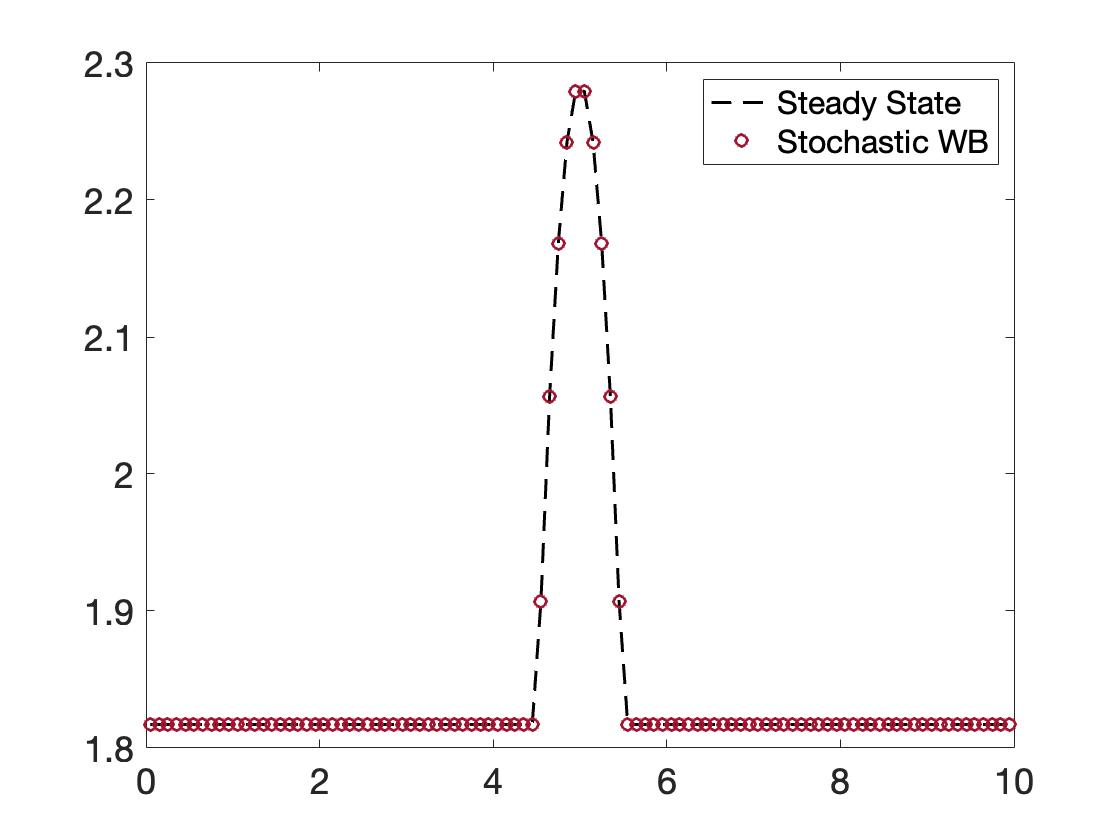
\includegraphics[width=0.85\textwidth]{./Figures/u4_wb_mean}
    \end{figure}
\end{frame}
\begin{frame}{Mean: $f(u) = u^4 / 4$}
    \begin{figure}
    \centering
    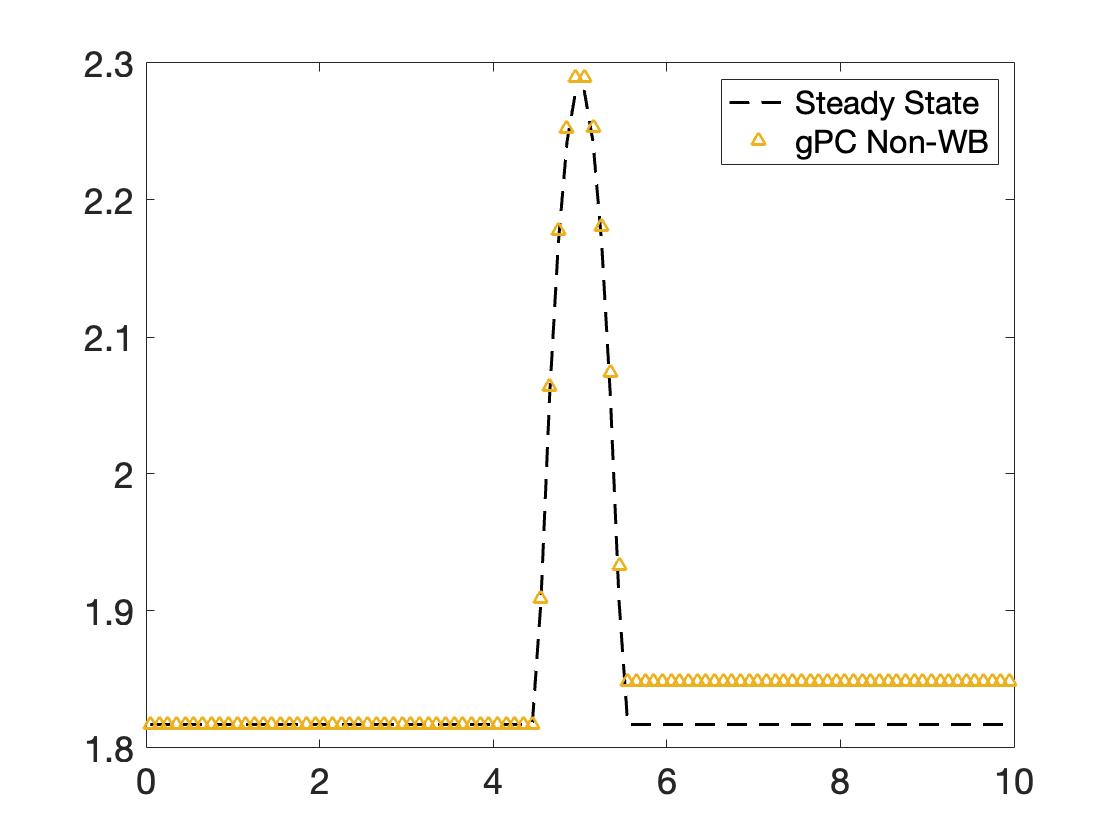
\includegraphics[width=0.85\textwidth]{./Figures/u4_non_mean}
    \end{figure}
\end{frame}

\begin{frame}{Standard Deviation: $f(u) = u^4 / 4$}
    \begin{figure}
    \centering
    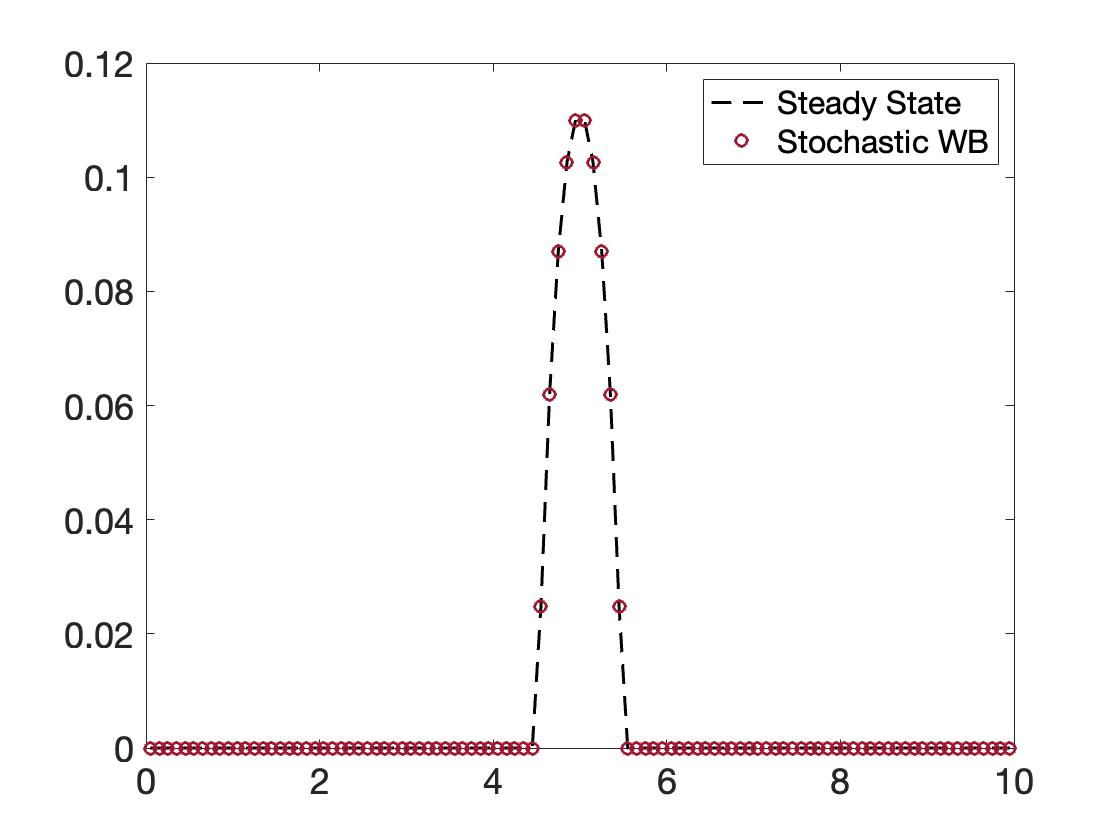
\includegraphics[width=0.85\textwidth]{./Figures/u4_wb_sd}
    \end{figure}
\end{frame}
\begin{frame}{Standard Deviation: $f(u) = u^4 / 4$}
    \begin{figure}
    \centering
    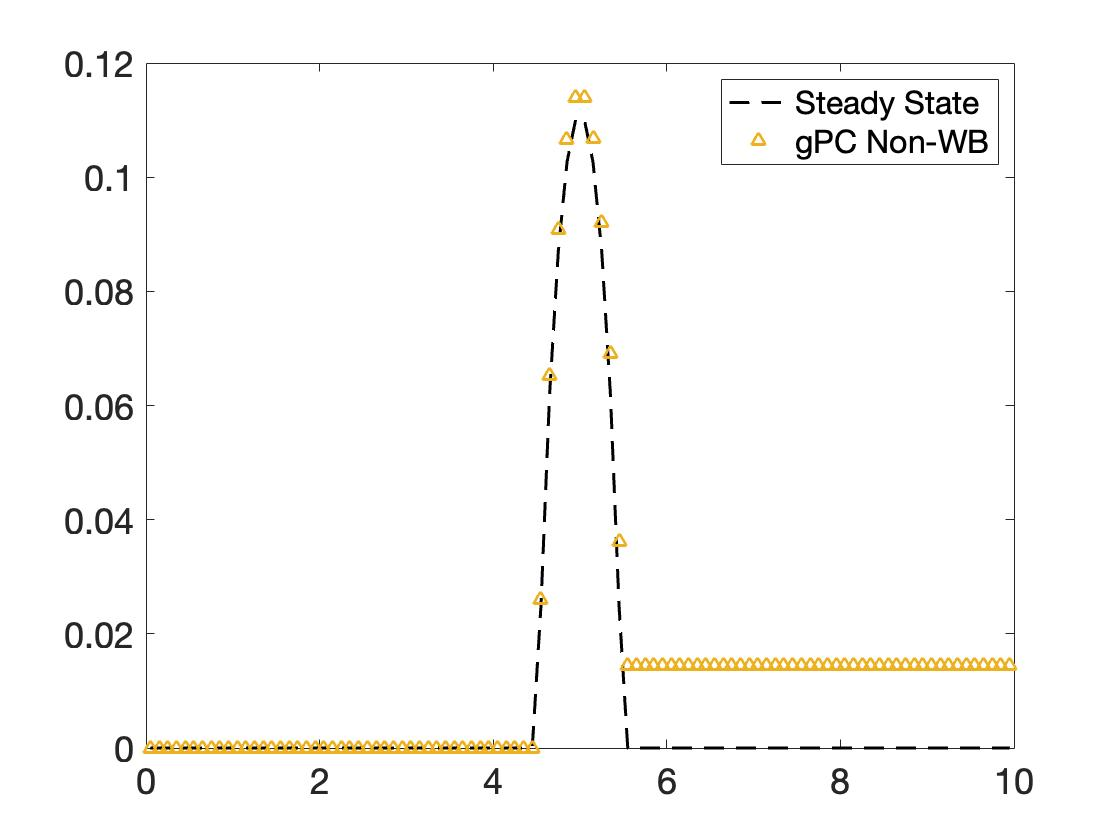
\includegraphics[width=0.85\textwidth]{./Figures/u4_non_sd}
    \end{figure}
\end{frame}

%%%%%%%%%%%%%%%%%%%%%%%%%%%%%%%%%%%%%%%%%%%%%%%%%%%%%%%%%%%%%%%%%%%%%%%%%%%%%%%
%%% Numerical Considerations
%%%%%%%%%%%%%%%%%%%%%%%%%%%%%%%%%%%%%%%%%%%%%%%%%%%%%%%%%%%%%%%%%%%%%%%%%%%%%%%
\section{Numerical Considerations}
\begin{frame}{Numerical Considerations}
   \begin{equation*}
       \partial_t \hat{\vb{u}}_j + \frac{\vb{A}_j \hat{\vb{u}}_j - \vb{A}_{j-1} \hat{\vb{u}}_{j-1}}{2\Delta x} = -\frac{(\vb{B}_j - \vb{B}_{j-1})(\hat{\vb{u}}_j + \hat{\vb{u}}_{j-1})}{2\Delta x}
   \end{equation*} 
   There are a couple of points to note regarding this scheme:
   \begin{itemize}
       \item $\hat{u}$ has $N_x \times M$ entries;
       \item $\vb{B}$ is constant in time $\implies$ can be computed before time evolution
       \item $\vb{A}$ depends on time $\implies$ must be computed per time step.
       \item $\vb{A}_j$ and $\vb{B}_j$ are symmetric.
   \end{itemize}
   Based on profiling, the computation of $\vb{A}$ dominates runtime. In the $f(u) = u^4 / 4$ scenario, $\vb{S}$ is extremely costly in the same way.
\end{frame}

%%%%%%%%%%%%%%%%%%%%%%%%%%%%%%%%%%%%%%%%%%%%%%%%%%%%%%%%%%%%%%%%%%%%%%%%%%%%%%%
%%% Discussion and Future Work
%%%%%%%%%%%%%%%%%%%%%%%%%%%%%%%%%%%%%%%%%%%%%%%%%%%%%%%%%%%%%%%%%%%%%%%%%%%%%%%
\section{Discussion}
\begin{frame}{Discussion}
   In summary, we've implemented a method which:
   \begin{itemize}
       \item Handles a random input in a physically derived forcing term
       \item Can be generalized to different forms of fluxes other than Burgers
       \item Is well-balanced in a stochastic sense
       \item Handles discontinuous solutions resulting from discontinuous forcing.
   \end{itemize}
\end{frame}

%%%%%%%%%%%%%%%%%%%%%%%%%%%%%%%%%%%%%%%%%%%%%%%%%%%%%%%%%%%%%%%%%%%%%%%%%%%%%%%
%%% References
%%%%%%%%%%%%%%%%%%%%%%%%%%%%%%%%%%%%%%%%%%%%%%%%%%%%%%%%%%%%%%%%%%%%%%%%%%%%%%%
\begin{frame}{References}
\printbibliography
\end{frame}

\end{document}